% \documentclass[11pt,a4]{aleph-examen}
\documentclass[11pt,respuestas,a4]{aleph-examen}

% -- Paquetes extra
\usepackage{aleph-comandos}
\usepackage{tikz}
\usetikzlibrary{calc,babel}
\usepackage{pgfplots}
\pgfplotsset{compat=1.17}

% -- Datos
\institucion{Facultad de Ciencias Exactas, Naturales y Ambientales}
\carrera{Catálogo STEM}
\asignatura{Matemática III}
\tema{Taller 01: Funciones vectoriales y geometría diferencial}
\autor{Andrés Merino}
\fecha{Periodo 2026-1}

\logouno[0.16\textwidth]{Logos/logoPUCE_04_ac}
\definecolor{colortext}{HTML}{1957d1}
\definecolor{colordef}{HTML}{1957d1}
\fuente{montserrat}

\begin{document}

\encabezado


\section*{Indicaciones}
\begin{itemize}[leftmargin=*]
\item
    En esta actividad se evalúa si el estudiante (Criterio 2.1) determina dominios de funciones de varias variables a través de su representación gráfica o su ley de asignación.
\item
    El taller se desarrolla en grupos de hasta 3 personas.
\item
    Se permite y se recomienda el uso de asistentes computacionales (GeoGebra, Python, Mathematica, etc.) para graficar y realizar cálculos; sin embargo, cada respuesta de análisis debe estar escrita y justificada por el grupo.
\item
    Las resoluciones deben entregarse de forma escrita en formato físico, con todos los procedimientos y gráficas claramente presentados.
\item
    Todas las conclusiones deben estar correctamente redactadas; no basta con presentar el resultado del asistente computacional.
\end{itemize}

%%%%%%%%%%%%%%%%%%%%%%%%%%%%%%%%%%%%%%%%%%
\begin{preguntas}

%%%%%%%%%%%%%%%%%%%%%%%%%%%%%%%%%%%%%%%%%%
\item
Considere la trayectoria
\[
    \funcion{\alpha}{[0,2\pi]}{\R^2}{t}{(\sen(2t),\;\sen(3t)).}
\]
\begin{enumerate}
    \item Evalúe la función en $0$, $1$, $\pi$, $2\pi$.
    \item Use un asistente computacional para graficar la curva. Incluya los resultados del literal anterior.
    \item Calcule $\alpha'(t)$ y determine todos los valores de $t\in[0,2\pi]$ para los que el vector tangente es horizontal ($\alpha_2'(t)=0$) o vertical ($\alpha_1'(t)=0$). ¿Qué ocurre geométricamente en esos puntos?
    \item La curva pasa varias veces por el origen. Encuentre todos los valores de $t$ para los que $\alpha(t)=(0,0)$. ¿Cuántos «cruces» ocurren?
\end{enumerate}

\begin{respuesta}\hspace{0pt}
\begin{enumerate}
    \item Evaluaciones:
    \begin{align*}
        \alpha(0)&=(\sen(0),\,\sen(0))=(0,0),\\
        \alpha(1)&=(\sen(2),\,\sen(3))\approx(0{,}9093,\;0{,}1411),\\
        \alpha(\pi)&=(\sen(2\pi),\,\sen(3\pi))=(0,0),\\
        \alpha(2\pi)&=(\sen(4\pi),\,\sen(6\pi))=(0,0).
    \end{align*}

    \item Gráfica:
    \begin{center}
    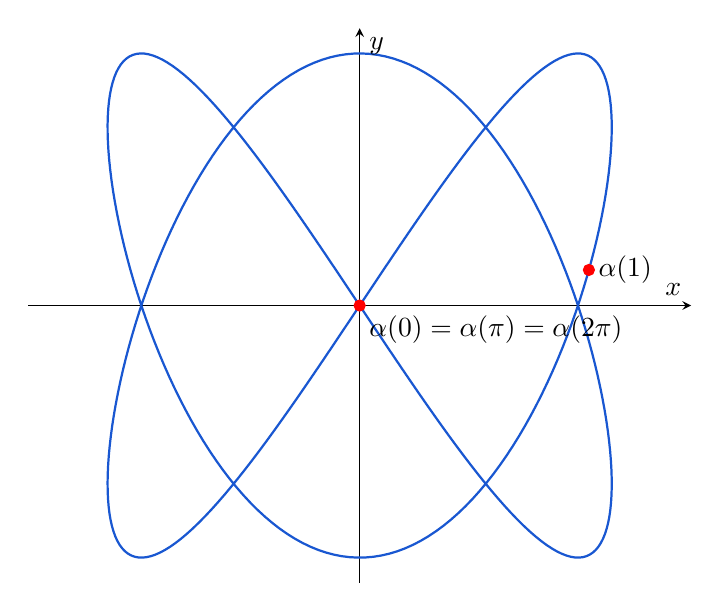
\begin{tikzpicture}
    \begin{axis}[width=10cm, axis equal, axis lines=middle,
        xlabel={$x$}, ylabel={$y$}, xmin=-1.1, xmax=1.1, ymin=-1.1, ymax=1.1, ticks=none]
        \addplot [colordef, thick, domain=0:2*pi, samples=400] ({sin(deg(2*x))}, {sin(deg(3*x))});
        % puntos evaluados
        \addplot[only marks, red, mark=*, mark size=2pt] coordinates {(0,0) (0.9093,0.1411)};
        \node[below right] at (axis cs:0,0) {$\alpha(0)=\alpha(\pi)=\alpha(2\pi)$};
        \node[right] at (axis cs:0.9093,0.1411) {$\alpha(1)$};
    \end{axis}
    \end{tikzpicture}
    \end{center}

    \item Derivada y tangentes:
    \[\alpha'(t)=(2\cos(2t),\;3\cos(3t)).\]
    El vector tangente es horizontal cuando $\alpha_2'(t)=3\cos(3t)=0$, es decir
    \[\cos(3t)=0\iff 3t=\tfrac{\pi}{2}+k\pi\iff t=\tfrac{\pi}{6}+\tfrac{k\pi}{3},\quad k\in\mathbb{Z}.
    \]
    Tomando $t\in[0,2\pi]$ obtenemos
    \[t=\tfrac{\pi}{6},\;\tfrac{\pi}{2},\;\tfrac{5\pi}{6},\;\tfrac{7\pi}{6},\;\tfrac{3\pi}{2},\;\tfrac{11\pi}{6}.
    \]
    El vector tangente es vertical cuando $\alpha_1'(t)=2\cos(2t)=0$, es decir
    \[\cos(2t)=0\iff 2t=\tfrac{\pi}{2}+k\pi\iff t=\tfrac{\pi}{4}+\tfrac{k\pi}{2},\quad k\in\mathbb{Z}.
    \]
    En $[0,2\pi]$ esto da
    \[t=\tfrac{\pi}{4},\;\tfrac{3\pi}{4},\;\tfrac{5\pi}{4},\;\tfrac{7\pi}{4}.
    \]
    Geométricamente, en los primeros valores la tangente es puramente horizontal (pendiente 0) y en los segundos puramente vertical.

    \item Cruces en el origen:
    Buscamos $\alpha(t)=(0,0)$, es decir $\sen(2t)=0$ y $\sen(3t)=0$. Esto ocurre cuando
    \[t=\tfrac{k\pi}{2}\quad\text{y}\quad t=\tfrac{m\pi}{3}.
    \]
    Los valores comunes en $[0,2\pi]$ son $t=0,\,\pi,\,2\pi$. Por tanto la curva pasa por el origen tres veces en el intervalo dado.\qedhere
\end{enumerate}
\end{respuesta}

%%%%%%%%%%%%%%%%%%%%%%%%%%%%%%%%%%%%%%%%%%
\item
Considere el campo escalar
\[
    \funcion{f}{\R^2\setminus\{(0,0)\}}{\R}{(x,y)}{2\sen\l(\sqrt{x^2+y^2}\r).}
\]
\begin{enumerate}
    \item Evalúe la función en $(0,0)$, $(1,1)$, $(0,\pi)$, $(\pi,0)$. 
    \item Use un asistente computacional para graficar la superficie $z=f(x,y)$. Incluya los resultados del literal anterior.
    \item Determine las curvas de nivel con $c=0$, $c=1$, $c=-1$, $c=2$, $c=-2$. Describa en palabras las curvas de nivel. Muestre un gráfico de las curvas de nivel usando colores para su mejor comprensión.
\end{enumerate}

\begin{respuesta}\hspace{0pt}
\begin{enumerate}
    \item El punto $(0,0)$ no pertenece al dominio de $f$. Para los demás puntos:
    \begin{align*}
        f(1,1)   &= 2\sen\!\l(\sqrt{1^2+1^2}\r) = 2\sen\!\l(\sqrt{2}\r) \approx 1{,}975,\\
        f(0,\pi) &= 2\sen\!\l(\sqrt{0^2+\pi^2}\r) = 2\sen(\pi) = 0,\\
        f(\pi,0) &= 2\sen\!\l(\sqrt{\pi^2+0^2}\r) = 2\sen(\pi) = 0.
    \end{align*}

    \item Gráfica:
    \begin{center}
    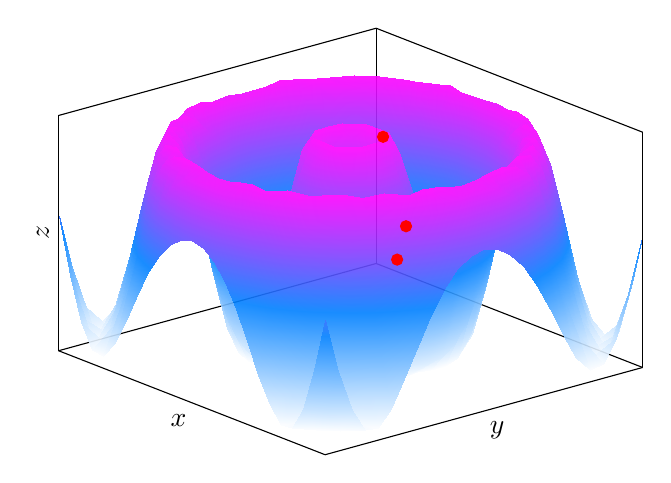
\begin{tikzpicture}
    \begin{axis}[
        view={50}{30}, width=9cm, height=7cm,
        xlabel={$x$}, ylabel={$y$}, zlabel={$z$},
        domain=-9:9, y domain=-9:9, samples=25,
        colormap/cool, zmin=-2.2, zmax=2.2, ticks=none
    ]
        \addplot3[surf, shader=interp, opacity=0.9]
            {2*sin(deg(sqrt(x^2+y^2)))};
        \addplot3[only marks, mark=*, mark options={fill=red, draw=red}, mark size=2pt]
            coordinates {(1,1,1.975) (0,3.14159,0) (3.14159,0,0)};
    \end{axis}
    \end{tikzpicture}
    \end{center}

    \item La ecuación de nivel $f(x,y)=c$ equivale a $\sen\!\l(\sqrt{x^2+y^2}\r)=c/2$.
    Llamando $r=\sqrt{x^2+y^2}$, las soluciones positivas son
    \[
        r = \arcsin\!\l(\tfrac{c}{2}\r)+2k\pi \quad\text{o}\quad
        r = \pi-\arcsin\!\l(\tfrac{c}{2}\r)+2k\pi, \qquad k=0,1,2,\ldots
    \]
    Cada valor de $r$ corresponde a una \textbf{circunferencia concéntrica} centrada en el origen. Los radios para los valores pedidos son:
    \begin{center}
    \begin{tabular}{|c|l|}
    \hline
    $c$ & Radios \\
    \hline
    $0$  & $\pi,\quad 2\pi,\quad 3\pi,\quad \ldots$ \\
    $2$  & $\tfrac{\pi}{2},\quad \tfrac{5\pi}{2},\quad \tfrac{9\pi}{2},\quad \ldots$ \\
    $-2$ & $\tfrac{3\pi}{2},\quad \tfrac{7\pi}{2},\quad \tfrac{11\pi}{2},\quad \ldots$ \\
    $1$  & $\tfrac{\pi}{6},\quad \tfrac{5\pi}{6},\quad \tfrac{\pi}{6}+2\pi,\quad \ldots$ \\
    $-1$ & $\tfrac{7\pi}{6},\quad \tfrac{11\pi}{6},\quad \tfrac{7\pi}{6}+2\pi,\quad \ldots$ \\
    \hline
    \end{tabular}
    \end{center}

    \begin{center}
    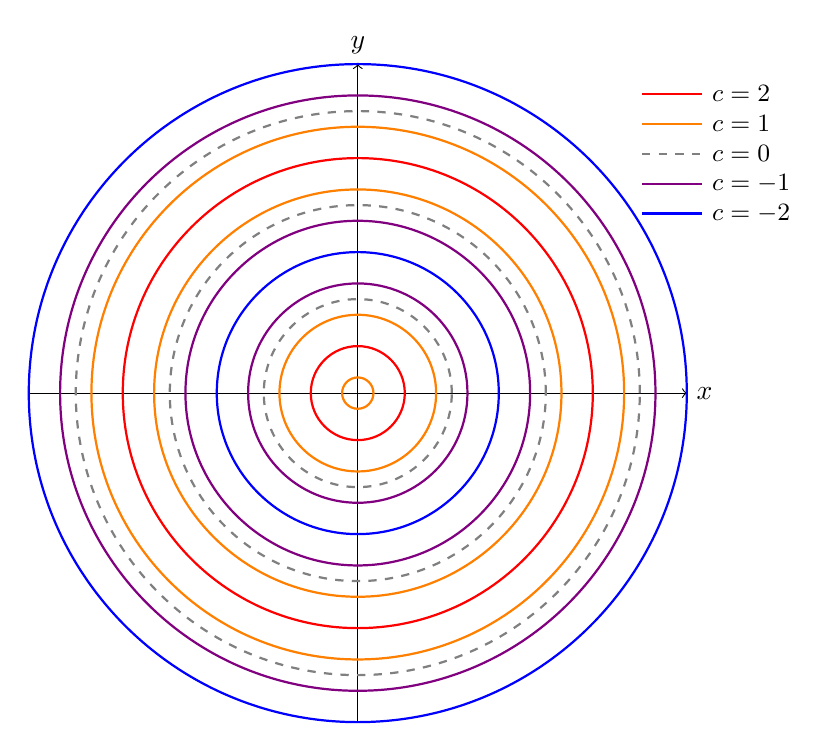
\begin{tikzpicture}[scale=0.38]
        \draw[->] (-11,0) -- (11,0) node[right] {$x$};
        \draw[->] (0,-11) -- (0,11) node[above] {$y$};
        % c=0  (r = pi, 2pi, 3pi)
        \draw[gray, dashed, thick] (0,0) circle (3.1416);
        \draw[gray, dashed, thick] (0,0) circle (6.2832);
        \draw[gray, dashed, thick] (0,0) circle (9.4248);
        % c=2  (r = pi/2, 5pi/2)
        \draw[red, thick] (0,0) circle (1.5708);
        \draw[red, thick] (0,0) circle (7.8540);
        % c=-2  (r = 3pi/2, 7pi/2)
        \draw[blue, thick] (0,0) circle (4.7124);
        \draw[blue, thick] (0,0) circle (10.9956);
        % c=1  (r = pi/6, 5pi/6, pi/6+2pi, 5pi/6+2pi)
        \draw[orange, thick] (0,0) circle (0.5236);
        \draw[orange, thick] (0,0) circle (2.6180);
        \draw[orange, thick] (0,0) circle (6.8068);
        \draw[orange, thick] (0,0) circle (8.9012);
        % c=-1  (r = 7pi/6, 11pi/6, 7pi/6+2pi)
        \draw[violet, thick] (0,0) circle (3.6652);
        \draw[violet, thick] (0,0) circle (5.7596);
        \draw[violet, thick] (0,0) circle (9.9484);
        % Leyenda
        \draw[red, thick]         (9.5,10) -- (11.5,10) node[right, black, font=\small] {$c=2$};
        \draw[orange, thick]       (9.5, 9) -- (11.5, 9) node[right, black, font=\small] {$c=1$};
        \draw[gray, dashed, thick] (9.5, 8) -- (11.5, 8) node[right, black, font=\small] {$c=0$};
        \draw[violet, thick]       (9.5, 7) -- (11.5, 7) node[right, black, font=\small] {$c=-1$};
        \draw[blue, thick]         (9.5, 6) -- (11.5, 6) node[right, black, font=\small] {$c=-2$};
    \end{tikzpicture}
    \end{center}

    Las curvas de nivel son \textbf{circunferencias concéntricas} centradas en el origen. La función oscila entre $-2$ y $2$, por lo que para cada $c\in(-2,2)$ existen infinitas curvas de nivel; para $c=\pm2$, cada curva de nivel consiste en circunferencias aisladas (donde $2\sen(r)$ alcanza su valor extremo).\qedhere
\end{enumerate}
\end{respuesta}

%%%%%%%%%%%%%%%%%%%%%%%%%%%%%%%%%%%%%%%%%%
\item
Considere el campo vectorial
\[
    \funcion{F}{\R^2\setminus\{(0,0)\}}{\R^2}{(x,y)}{\l(\dfrac{-y}{x^2+y^2},\;\dfrac{x}{x^2+y^2}\r).}
\]
\begin{enumerate}
    \item Evalúe la función en $(1,1)$, $(1,0)$, $(0,1)$, $(-1,0)$, $(0,-1)$, $(-1,-1)$. 
    \item Use un asistente computacional para graficar el campo vectorial $F$. Incluya los resultados del literal anterior.
    \item A partir de la gráfica, describa en palabras el comportamiento de las líneas de campo. ¿Qué fenómeno físico podría modelar este campo?
\end{enumerate}

\begin{respuesta}\hspace{0pt}
\begin{enumerate}
    \item Se evalúa $F(x,y)=\l(\dfrac{-y}{x^2+y^2},\;\dfrac{x}{x^2+y^2}\r)$ en cada punto:
    \begin{align*}
        F(1,1)   &= \l(\tfrac{-1}{2},\;\tfrac{1}{2}\r), &
        F(1,0)   &= (0,\;1), \\
        F(0,1)   &= (-1,\;0), &
        F(-1,0)  &= (0,\;-1), \\
        F(0,-1)  &= (1,\;0), &
        F(-1,-1) &= \l(\tfrac{1}{2},\;-\tfrac{1}{2}\r).
    \end{align*}
    Nótese que $\|F(x,y)\|=\dfrac{1}{\sqrt{x^2+y^2}}$ y que $F(x,y)\perp(x,y)$ en todo punto del dominio.

    \item Las líneas punteadas indican las líneas de campo; los puntos rojos corresponden a las evaluaciones del literal anterior.
    \begin{center}
    \begin{tikzpicture}
    \begin{axis}[
        width=8cm, height=8cm, axis equal,
        axis lines=middle,
        xlabel={$x$}, ylabel={$y$},
        xmin=-3, xmax=3, ymin=-3, ymax=3,
        xtick={-2,-1,1,2}, ytick={-2,-1,1,2},
        tick label style={font=\scriptsize}
    ]
        % Líneas de campo (circunferencias)
        \addplot[dashed, gray!70, domain=0:360, samples=80, smooth]
            ({0.7*cos(x)}, {0.7*sin(x)});
        \addplot[dashed, gray!70, domain=0:360, samples=80, smooth]
            ({1.4*cos(x)}, {1.4*sin(x)});
        \addplot[dashed, gray!70, domain=0:360, samples=80, smooth]
            ({2.1*cos(x)}, {2.1*sin(x)});
        % Campo vectorial normalizado
% \addplot[
%     mesh,
%     colordef,
%     -stealth,
%     line width=0.5pt,
%     quiver={
%         u={-y/sqrt(x^2+y^2+0.001)},
%         v={ x/sqrt(x^2+y^2+0.001)},
%         scale arrows=0.18
%     },
%     samples=8,
%     samples y=8,
%     domain=-2.5:2.5,
%     y domain=-2.5:2.5
% ]
% (x,y);
        % Puntos del literal a)
        \addplot[only marks, mark=*, red, mark size=2pt]
            coordinates {(1,1) (1,0) (0,1) (-1,0) (0,-1) (-1,-1)};
    \end{axis}
    \end{tikzpicture}
    \end{center}

    \item En cada punto, el vector $F(x,y)$ es \textbf{perpendicular al vector posición} $(x,y)$ y apunta en sentido antihorario. Las \textbf{líneas de campo son circunferencias concéntricas} centradas en el origen, recorridas en sentido antihorario. La magnitud $\|F\|=1/r$ decrece con la distancia $r$ al origen, de modo que las flechas son más largas cerca del origen y más cortas lejos de él.

    Este campo puede modelar:
    \begin{itemize}
        \item La \textbf{velocidad de un vórtice puntual} en mecánica de fluidos (flujo bidimensional irrotacional excepto en el origen).
        \item El \textbf{campo magnético} generado por un conductor recto e infinito que lleva corriente en la dirección $z$ (Ley de Biot-Savart).
    \end{itemize}
\end{enumerate}
\end{respuesta}

%%%%%%%%%%%%%%%%%%%%%%%%%%%%%%%%%%%%%%%%%%
\item
La {astroide} es la curva plana descrita por
\[
    \funcion{\alpha}{[0,2\pi]}{\R^2}{t}{(\cos^3 t,\;\sen^3 t).}
\]
\begin{enumerate}
    \item Grafique la astroide con un asistente computacional. 
    \item Calcule $\alpha'(t)$ y determine los valores de $t$ donde $\alpha'(t)=\vec{0}$. ¿Qué representan estos puntos en la gráfica?
    \item Calcule $\|\alpha'(t)\|$ y simplifique la expresión para $t\in(0,\pi/2)$.
    \item Calcule la longitud del arco de la astroide en el primer cuadrante, es decir,
    \[
        L_1 = \int_0^{\pi/2}\|\alpha'(t)\|\,dt.
    \]
    \item Usando la simetría de la curva, determine la longitud total de la astroide.
\end{enumerate}

\begin{respuesta}\hspace{0pt}
\begin{enumerate}
    \item La astroide tiene cuatro cúspides en $(\pm1,0)$ y $(0,\pm1)$.
    \begin{center}
    \begin{tikzpicture}[scale=2.3]
        \draw[->] (-1.3,0) -- (1.3,0) node[right] {$x$};
        \draw[->] (0,-1.3) -- (0,1.3) node[above] {$y$};
        \foreach \x in {-1,1}
            \draw (\x,0.03) -- (\x,-0.03) node[below, font=\scriptsize] {$\x$};
        \foreach \y in {-1,1}
            \draw (0.03,\y) -- (-0.03,\y) node[left, font=\scriptsize] {$\y$};
        \draw[colordef, thick, domain=0:360, samples=200, variable=\t]
            plot ({(cos(\t))^3}, {(sin(\t))^3});
        \filldraw[red] ( 1, 0) circle (0.025) node[below right, font=\scriptsize] {$(1,0)$};
        \filldraw[red] ( 0, 1) circle (0.025) node[above right, font=\scriptsize] {$(0,1)$};
        \filldraw[red] (-1, 0) circle (0.025) node[below left,  font=\scriptsize] {$(-1,0)$};
        \filldraw[red] ( 0,-1) circle (0.025) node[below right, font=\scriptsize] {$(0,-1)$};
    \end{tikzpicture}
    \end{center}

    \item La derivada es
    \[
        \alpha'(t) = \bigl(-3\cos^2 t\,\sen t,\; 3\sen^2 t\,\cos t\bigr).
    \]
    Se tiene $\alpha'(t)=\vec{0}$ si y solo si ambas componentes son cero. La primera se anula cuando $\cos t=0$ o $\sen t=0$; revisando la segunda en cada caso:
    \begin{itemize}
        \item $\sen t=0$: primera componente $=0$ ✓ y segunda $= 3\cdot 0\cdot\cos t=0$ ✓.
        \item $\cos t=0$: primera componente $=0$ ✓ y segunda $= 3\sen^2 t\cdot 0=0$ ✓.
    \end{itemize}
    En $[0,2\pi]$ se obtiene $t\in\{0,\,\pi/2,\,\pi,\,3\pi/2,\,2\pi\}$, correspondiendo a los cuatro puntos $(\pm1,0)$ y $(0,\pm1)$. Estos son las \textbf{cúspides} de la astroide: la curva llega a esos puntos con velocidad cero y no tiene tangente bien definida.

    \item Se calcula:
    \begin{align*}
        \|\alpha'(t)\|^2 &= 9\cos^4 t\,\sen^2 t + 9\sen^4 t\,\cos^2 t \\
                         &= 9\cos^2 t\,\sen^2 t\underbrace{(\cos^2 t+\sen^2 t)}_{=1} = 9\cos^2 t\,\sen^2 t,
    \end{align*}
    por lo tanto $\|\alpha'(t)\| = 3\,|\cos t\,\sen t| = \dfrac{3}{2}|\sen(2t)|$.

    Para $t\in(0,\pi/2)$, $\cos t>0$ y $\sen t>0$, de modo que
    \[
        \|\alpha'(t)\| = \frac{3}{2}\sen(2t).
    \]

    \item Integrando directamente:
    \[
        L_1 = \int_0^{\pi/2}\frac{3}{2}\sen(2t)\,dt
            = \frac{3}{2}\Bigl[-\frac{\cos(2t)}{2}\Bigr]_0^{\pi/2}
            = \frac{3}{4}\bigl[-\cos\pi+\cos 0\bigr]
            = \frac{3}{4}(1+1) = \frac{3}{2}.
    \]

    \item La astroide es simétrica respecto a los dos ejes coordenados, por lo que los cuatro arcos (uno por cuadrante) tienen la misma longitud. La longitud total es
    \[
        L = 4L_1 = 4\cdot\frac{3}{2} = 6.\qedhere
    \]
\end{enumerate}
\end{respuesta}

%%%%%%%%%%%%%%%%%%%%%%%%%%%%%%%%%%%%%%%%%%
\item
Considere la curva espacial
\[
    \funcion{\alpha}{[0,2\pi]}{\R^3}{t}{(\cos t,\;\sen t,\;\sen(2t)).}
\]
\begin{enumerate}
    \item Use un asistente computacional para graficar la curva en $\R^3$.
    \item Calcule $\alpha'(t)$, $\alpha''(t)$ y $\alpha'''(t)$.
    \item Calcule la curvatura.
    \item Use un asistente computacional para graficar $\kappa(t)$ en el intervalo $[0,2\pi]$.
    \item Determine los valores de $t\in[0,2\pi]$ donde la curvatura alcanza su valor máximo. Identifique los puntos correspondientes sobre la curva.
    \item Calcule la torsión.
\end{enumerate}

\begin{respuesta}\hspace{0pt}
\begin{enumerate}
    \item La curva está contenida en el cilindro unitario \(x^2+y^2=1\), con oscilación vertical dada por \(\sen(2t)\).

    \begin{center}
    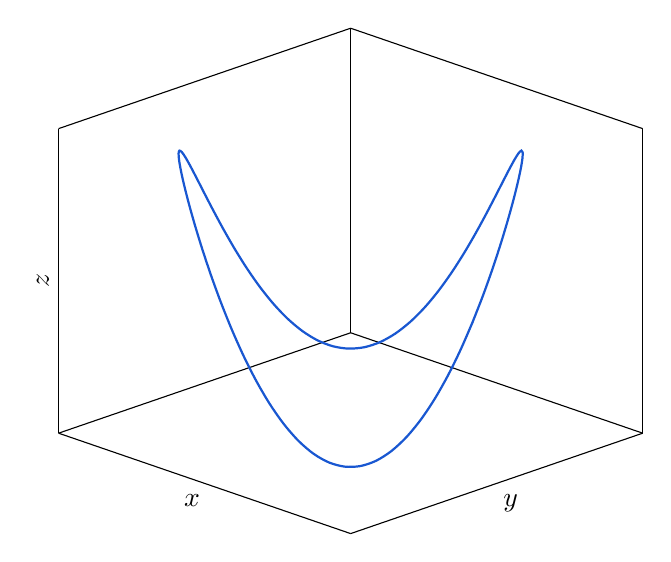
\begin{tikzpicture}
    \begin{axis}[
        view={45}{25},
        width=9cm,
        height=8cm,
        xlabel={$x$},
        ylabel={$y$},
        zlabel={$z$},
        xmin=-1.2, xmax=1.2,
        ymin=-1.2, ymax=1.2,
        zmin=-1.2, zmax=1.2,
        ticks=none
    ]
        \addplot3[
            colordef,
            thick,
            domain=0:2*pi,
            samples=70,
            variable=t,
            smooth
        ]
        ({cos(deg(t))}, {sin(deg(t))}, {sin(deg(2*t))});
    \end{axis}
    \end{tikzpicture}
    \end{center}

    \item Las derivadas son
    \begin{align*}
        \alpha'(t)   &= (-\sen t,\;\cos t,\;2\cos(2t)),\\
        \alpha''(t)  &= (-\cos t,\;-\sen t,\;-4\sen(2t)),\\
        \alpha'''(t) &= (\sen t,\;-\cos t,\;-8\cos(2t)).
    \end{align*}

    \item La curvatura viene dada por
    \[
        \kappa(t)
        =
        \frac{\|\alpha'(t)\times\alpha''(t)\|}{\|\alpha'(t)\|^3}.
    \]
    Como
    \[
        \alpha'(t)\times\alpha''(t)
        =
        \bigl(
            -2\sen t(2\cos^2t+1),
            -2\cos t(2\sen^2t+1),
            1
        \bigr),
    \]
    se tiene
    \[
        \|\alpha'(t)\times\alpha''(t)\|^2
        =
        12\sen^2(2t)+5,
    \]
    y
    \[
        \|\alpha'(t)\|^2
        =
        1+4\cos^2(2t).
    \]
    Por tanto,
    \[
        \kappa(t)
        =
        \frac{\sqrt{12\sen^2(2t)+5}}
        {\bigl(1+4\cos^2(2t)\bigr)^{3/2}}.
    \]

    \item Para hallar el máximo, escribimos
    \[
        \kappa^2(t)
        =
        \frac{17-12u}{(1+4u)^3},
        \qquad
        u=\cos^2(2t)\in[0,1].
    \]
    Entonces
    \[
        \frac{d}{du}\left(\kappa^2\right)
        =
        \frac{96u-216}{(1+4u)^4}<0,
        \qquad u\in[0,1].
    \]
    Por tanto, \(\kappa^2\) es decreciente respecto de \(u\), y su máximo ocurre cuando \(u=0\). Es decir,
    \[
        \cos(2t)=0.
    \]
    Luego,
    \[
        t\in
        \left\{
            \frac{\pi}{4},
            \frac{3\pi}{4},
            \frac{5\pi}{4},
            \frac{7\pi}{4}
        \right\}.
    \]
    El valor máximo de la curvatura es
    \[
        \kappa_{\max}=\sqrt{17}.
    \]

    Los puntos correspondientes son
    \begin{align*}
        \alpha\left(\frac{\pi}{4}\right)
        &=
        \left(
            \frac{\sqrt{2}}{2},
            \frac{\sqrt{2}}{2},
            1
        \right),
        &
        \alpha\left(\frac{3\pi}{4}\right)
        &=
        \left(
            -\frac{\sqrt{2}}{2},
            \frac{\sqrt{2}}{2},
            -1
        \right),
        \\
        \alpha\left(\frac{5\pi}{4}\right)
        &=
        \left(
            -\frac{\sqrt{2}}{2},
            -\frac{\sqrt{2}}{2},
            1
        \right),
        &
        \alpha\left(\frac{7\pi}{4}\right)
        &=
        \left(
            \frac{\sqrt{2}}{2},
            -\frac{\sqrt{2}}{2},
            -1
        \right).
    \end{align*}

    \item La torsión viene dada por
    \[
        \tau(t)
        =
        \frac{(\alpha'(t)\times\alpha''(t))\cdot\alpha'''(t)}
        {\|\alpha'(t)\times\alpha''(t)\|^2}.
    \]
    Como
    \[
        (\alpha'(t)\times\alpha''(t))\cdot\alpha'''(t)
        =
        -6\cos(2t),
    \]
    se obtiene
    \[
        \tau(t)
        =
        \frac{-6\cos(2t)}{12\sen^2(2t)+5}.
    \]
\end{enumerate}
\end{respuesta}

\end{preguntas}

\end{document}
